\documentclass[12pt]{article}

\usepackage{fullpage}
\usepackage{graphicx, rotating, booktabs} 
\usepackage{times} 
\usepackage{natbib} 
\usepackage{indentfirst} 
\usepackage{setspace}
\usepackage{grffile} 
\usepackage{hyperref}
\usepackage{adjustbox}
\setcitestyle{aysep{}}


\singlespace
\title{
\textbf{Reassessing the Public Goods Theory of Alliances}
	}
\author{Joshua Alley\footnote{Postdoctoral Research Associate,
Democratic Statecraft Lab, University of Virginia.}}
\date{{\normalsize \today}}

\bibliographystyle{apsr}

\begin{document}

\maketitle 

\doublespace

\begin{abstract}
The public goods theory of alliances exerts substantial influence on scholarship and policy, especially through its claim that small alliance participants free-ride on larger partners. 
Prior statistical tests of free-riding suffer from model specification and generalizability problems, however, so there is little reliable and general evidence about this prediction.
In this study, I address those limitations with a new test of the free-riding hypothesis. 
Using data on 204 alliances from 1919 to 2007, I examine how often states with a small share of total GDP in an alliance decrease military spending while states with a large share of allied GDP increase military spending. 
I find little evidence to support this expression of the free-riding hypothesis. 
This implies that free-riding based on economic weight is unusual in alliance politics, which may be due to limits on alliance security as a public good or bargaining between alliance members. 
\end{abstract} 

\newpage


%----------------------------------
\section{Introduction}



\citet{OlsonZeckhauser1966} argue that international alliances generate a collective action problem. 
According to their theory, security from an alliance is a public good, so smaller alliance participants ``free ride'' on the contributions of larger members. 
Free-riding is reflected by disproportionate allocations of resources to defense, where smaller alliance members spend a lower share of their national income on the military, relative to larger partners.


% So what am I doing here?: revisiting is necessary. 
\textbf{
The prominence of the public goods model in academic and policy discussions of alliances belies a major problem.
Fifty-three years after the publication of ``An Economic Theory of Alliances,'' there is little reliable and general evidence about Olson and Zeckhauser's prediction that small states are prone to free-ride. 
Here, I attempt to fill that empirical gap in the literature. 
}

\textbf{
In this paper, I test the free-riding prediction with a statistical model that addresses model specification and generalizability issues in previous research. 
I use the public goods logic to predict that states with a low share of total GDP in an alliance will decrease percentage changes in military spending, and states with high share of total allied GDP will increase military spending.
Then I employ a Bayesian model to estimate the association between economic weight and percentage changes in military spending for 204 alliances. 
I find little evidence of free-riding based on economic weight.
}


My research design addresses two key limitations in existing tests of the public goods logic.
First, many empirical estimates of free-riding within alliances have a model specification problem with the dependent variable.
Olson and Zeckhauser use military spending as a share of GDP to measure contributions to the alliance, and GDP to measure state size.
This approach is widely emulated, but it is problematic because GDP is part of the independent and dependent variables.
Changes in GDP shift the defense burden, and this deterministic component affects correlation and regression estimates.\footnote{See the appendix for a formal demonstration of this claim.}  


One notable paper addresses the dependent variable specification problem, but may not produce general findings. 
\citet{PluemperNeumayer2015} examine how growth in military spending by North Atlantic Treaty Organization (NATO) members responds to changing US and Soviet spending.
They demonstrate that NATO members are unresponsive to US and Soviet military spending, and present this as evidence of free riding.
\citet{PluemperNeumayer2015} also find no correlation between NATO member size and the extent of free-riding, however, which they argue contradicts \citet{OlsonZeckhauser1966}.
This paper's focus on NATO brings me to the second limitation: a lack of generalizability. 


% Huge (over)emphasis on NATO 
NATO is the epicenter of free-riding discussions. 
Following Olson and Zeckhauser's emphasis on military spending as a share of GDP, accusations of free-riding emphasize that NATO members have lower defense burdens than the United States. 
Scholars, pundits and policymakers have spent decades arguing over how well the public goods model applies to NATO, e.g. \citep{Pryor1968, SandlerForbes1980, Palmer1990, HiltonVhu1991, Boyer1993, GatesTerasawa1992, SandlerHartley2001, Lanoszka2015, PluemperNeumayer2015, KimSandler2019}.


% So what is the problem here?: it's mostly NATO
Most studies of the public goods model focus on NATO, but NATO is a difficult case for making general conclusions. 
NATO is exceptionally large, durable and capable. 
There are only seven tests of the public goods model outside of NATO, most of which examine one or two alliances \citep{Russett1970, Starr1974, Reisinger1983, Thies1987, ConybeareSandler1990, OnealWhatley1996, Siroky2012}. 
Six of these studies estimate correlations between GDP and defense burdens, so they suffer from the aforementioned specification problem.
This leaves a need for a general examination of the public goods logic. 


% I'm not the first one to address this theory: first comprehensive empirical evidence
Using a Bayesian model that estimates the association between economic weight and percentage changes in military spending within many alliances, I find little evidence that small states are more inclined to free-ride than their larger allies.
\textbf{This finding expands the economic size results of \citet{PluemperNeumayer2015} from the NATO case.}
Given established theoretical skepticism of the public goods model e.g. \citep{Palmer1990, GatesTerasawa1992, SandlerHartley2001, Norrlof2010, NiouZeigler2019}, what do these findings add? 
Some existing theoretical skepticism of the public goods model is motivated by inconsistent correlations between GDP and defense burdens. 
These correlations do not provide reliable evidence, however. 
Without a reliable and general test, theoretical revisions of a parsimonious public goods model may be premature.

\textbf{
There are three reasons to undertake another test of the public goods model. 
First, although academic theory has progressed since 1966, the public goods model retains an important place in discourse about alliances e.g.,\citep{Walt1990, Sandler1993, Mearsheimer1994, Goldstein1995, SandlerHartley2001, Garfinkel2004, Walt2009, Norrlof2010, Barrett2010, PluemperNeumayer2015}.
Second, policy and popular discussions of alliances employ collective action ideas.
Pundits and American policymakers often refer to allied ``free-riding'' \citep{Lanoszka2015}.   
For example, Barack Obama complained in 2016 that ``Free riders aggravate me'' and US allies ``have to pay your fair share.'' 
Donald Trump has implied that the United States would not protect allies who spend too little on defense. 
}

% this is the spot for frame on benefits and burdens of US Alliances 
\textbf{
Third, increasing great power competition makes assessing Olson and Zeckhauser's argument important for policy debates. 
Competing visions of US grand strategy hinge in part on the explanatory power of the public goods model. 
Advocates of retrenchment and ``restraint'' use the public goods logic to claim that US allies free-ride, so the United States should withdraw from many alliances \citep{Preble2009, Posen2014}. 
Others assert that alliances do not provide a public good and the benefits of alliance participation outweigh the costs \citep{Brooksetal2013, BrandsFeaver2017}. 
}

The paper proceeds as follows.
First, I briefly summarize the public goods theory of alliances.
Then I describe the model and results. 
In the final section, I discuss some implications of the findings for scholarship and policy. 



\section{Free-Riding in Alliances}

% I do not test their exact proposition 
\textbf{
To identify observable implications of free-riding, I use the public goods argument to derive predictions about economic size and military spending in alliances.
This exercise does not critique the public goods model.
Instead, I take the public goods logic as given, but employ another measure of defense effort. 
Following \citet{PluemperNeumayer2015} I use percentage changes in military spending to measure defense effort.
Like Olson and Zeckhauser, I conceptualize state size using economic weight. 
}

% summarize argument
\textbf{
Olson and Zeckhauser connect alliances and defense spending through a collective action problem. 
As the aggregate military capability of an alliance provides security for members, states contribute security by investing in their military.
Because an alliance cannot exclude members without undermining its purpose, alliance security is a public good. 
Olson and Zeckhauser expect that larger members of the alliance will invest more in defense, because these states value security from the alliance more.
Small alliance members rely on larger partners for security and reduce their defense burdens.
As a result, small states free-ride on larger alliance participants. 
%Moreover, small states have greater bargaining leverage, because a large state cannot credibly threaten to reduce their contribution and has ``relatively less to gain than its small ally from driving a hard bargain'' \citep[pg. 274]{OlsonZeckhauser1966}. 
}


% Economic weight as another way to get at O+Z's key comparion
Olson and Zeckhauser compare alliance member size using economic resources, specifically GDP.
Economic weight within an alliance, or each state's share of total allied GDP, is a related way to conceptualize differences in state size.
Using economic weight facilitates state size comparisons across diverse alliances, where states may be large or small members. 
A greater share of total economic resources in an alliance gives a state more economic weight and increases their potential military spending contribution. 


In the public goods model, economic weight shapes defense expenditures. 
Smaller members can free-ride and lower military spending. 
Because larger states place higher absolute value on security from an alliance, alliance participation will increase their investment in military capability. 
Therefore, alliance participation will decrease military spending by small states and increase military spending by large states. 


% Clarify that both predictions approximate the O+Z logic
I test the public goods predictions of military spending by small and large alliance members in a sample of all non-microstates from 1919 to 2007, using percentage changes in spending to facilitate a reliable and general empirical test.\footnote{Limited GDP data makes constructing economic weights for each alliance difficult before 1919. I also omit some alliances after 1919 due to a lack of GDP data.}
State-year observations are the unit of analysis.
My assessment of the public goods model estimates the extent of free-riding within individual alliances using alliance-specific economic weight parameters.  
 

\section{Testing the Public Goods Logic}


\textbf{
I use a Bayesian model to estimate alliance-specific effects of differences in economic weight on military spending.\footnote{I also make similar inferences by regressing percentage changes in military spending on a state's average weight in their alliances and with a model of changes in spending. See the appendix.}
This approach provides general evidence about the association between economic weight and military spending across 204 alliances.
I use Bayesian estimation because it regularizes the 204 alliance parameter estimates.
Partial pooling in this Bayesian model draws on information from all alliances to inform each alliance parameter estimate.\footnote{I fit the following model using STAN \citep{Carpenteretal2016}. See the appendix for a full summary of priors, convergence and model fit. I also show that the model recovers known parameters from simulated data.}
With hundreds of alliance-specific parameters, Bayesian estimation shares information across alliance parameters with less risk of spurious inferences from multiple comparisons. 
}


For each of the 204 ATOP offensive and defensive treaties \citep{Leedsetal2002}, I estimate the association between economic weight and military expenditures. 
An economic weight parameter for each alliance captures the consequences of alliance participation for military spending. 
I code economic weight in alliances such that a positive economic weight parameter implies more military spending for large members and less spending by small members, as the public goods model predicts. 
A negative economic weight parameter indicates that larger alliance members spend less on the military, and small members spend more. 


The model starts with state-year percentage changes in military spending $y_{it}$, transformed with an inverse hyperbolic sine.\footnote{\textbf{This transformation pulls in large positive and negative percentage changes to reduce the impact of outliers on the results.}} 
I model this variable using a t-distribution with degrees of freedom $\nu$ to account for heavy tails.
The expected value of military spending $\mu_{it}$ depends on a constant $\alpha$, state and year varying intercepts, and state-year control variables $\mathbf{X_{it}} \beta$.\footnote{See the appendix for a full description of all the variables in the model, as well as an explanation of the priors.} 
$\sigma$ captures unexplained variation in $y$, like the error term in a frequentist regression. 

\begin{equation}
y_{it} \sim student_t(\nu, \mu_{it}, \sigma) 
\end{equation}

\begin{equation}
\mu_{it} = \alpha + \alpha^{st} + \alpha^{yr} + \mathbf{X_{it}} \beta + \mathbf{Z_{it}} \gamma
\end{equation}


The $\mathbf{Z_{it}} \gamma$ term captures the impact of economic weight in alliances.  
$\textbf{Z}$ is a matrix of state participation in alliances--- columns are alliances, rows are state-year observations.  
If a state is part of an alliance, the corresponding element in $\textbf{Z}$ depends on their share of total GDP in the alliance. 
I assigned small alliance members a value of negative one if their economic weight is less than .5 in bilateral alliances, or less than .08 in multilateral alliances.
Large alliance members have a value of positive one in $\textbf{Z}$ if their economic weight is above those thresholds. 
Having more than half of GDP in a bilateral pact is a clear threshold for asymmetry. 
I set the threshold to the third quartile of .08 in multilateral alliances because the distribution of economic weight is very different in those alliances. 
Increasing the multilateral threshold would classify even the US in NATO as a small state, so .08 is a reasonable value. 
If a state is not part of the alliance, the corresponding matrix element is zero.

\textbf{ 
This coding of economic weight facilitates a simple test of the public goods hypothesis across multiple alliances. 
Multiplying a positive $\gamma$ by negative one for small states reduces military spending growth.
Multiplying the same positive economic weight parameter by positive one increases military spending growth for large states. 
Therefore, positive $\gamma$ parameters will change military spending growth in ways that match the public goods model. 
}

$\textbf{Z}$ is a quasi-spatial approach to capturing the impact of participation in multiple alliances.
In this model, alliance participation affects military spending through economic weight.  
The $\gamma$ parameters capture whether differences in economic weight between alliance members drive differences in military spending. 


$\gamma$ is a vector of 204 alliance-specific economic weight parameters.  
\textbf{Because \textbf{Z} contains a binary encoding of each state's share of allied GDP, the $\gamma$ coefficients estimate the association between a state's economic weight in an alliance and military spending.}\footnote{This assumes symmetric effects across small and large states, which I relax in the appendix with a weighted coding of the economic weights in $\textbf{Z}$.} 
When a state is not in an alliance, the corresponding $\gamma$ is multiplied by zero, and has no impact. 


Each alliance has unique effects on military spending, but the economic weight parameters have a common prior distribution where $\gamma \sim N(\theta, \sigma_{all})$, which shares information across the alliance estimates. 
Partial pooling estimates the dispersion of the alliance parameters from the data, so the prior for $\gamma$ has mean $\theta$ and variance $\sigma_{all}$, and relies on a normal distribution, which is standard in most multilevel models.  
$\theta$ is the mean hyperparameter of the alliance coefficients and each $\gamma$ deviates from the overall mean $\theta$ based on a variance hyperparameter $\sigma_{all}$.
Every economic weight parameter holds the impact of other alliances constant. 
    


\subsection{Results} 


The public goods model predicts many positive economic weight parameters. 
Because I employed Bayesian modeling, each $\gamma$ has a posterior distribution.
I focus interpretation on the posterior mean and 90\% credible intervals.\footnote{I use 90\% credible intervals because inferences around 95\% intervals are unstable.}
The posterior mean is the expected value of $\gamma$, while the credible intervals capture uncertainty around that estimate.  


No alliance has a clear positive economic weight parameter.
\autoref{fig:alliance-coefs-year} plots the $\gamma$ parameter for each alliance against the start year of the treaty.
Points mark the posterior mean. 
The error bars encapsulate the 90\% credible interval.


\begin{figure}[htbp]
	\centering
		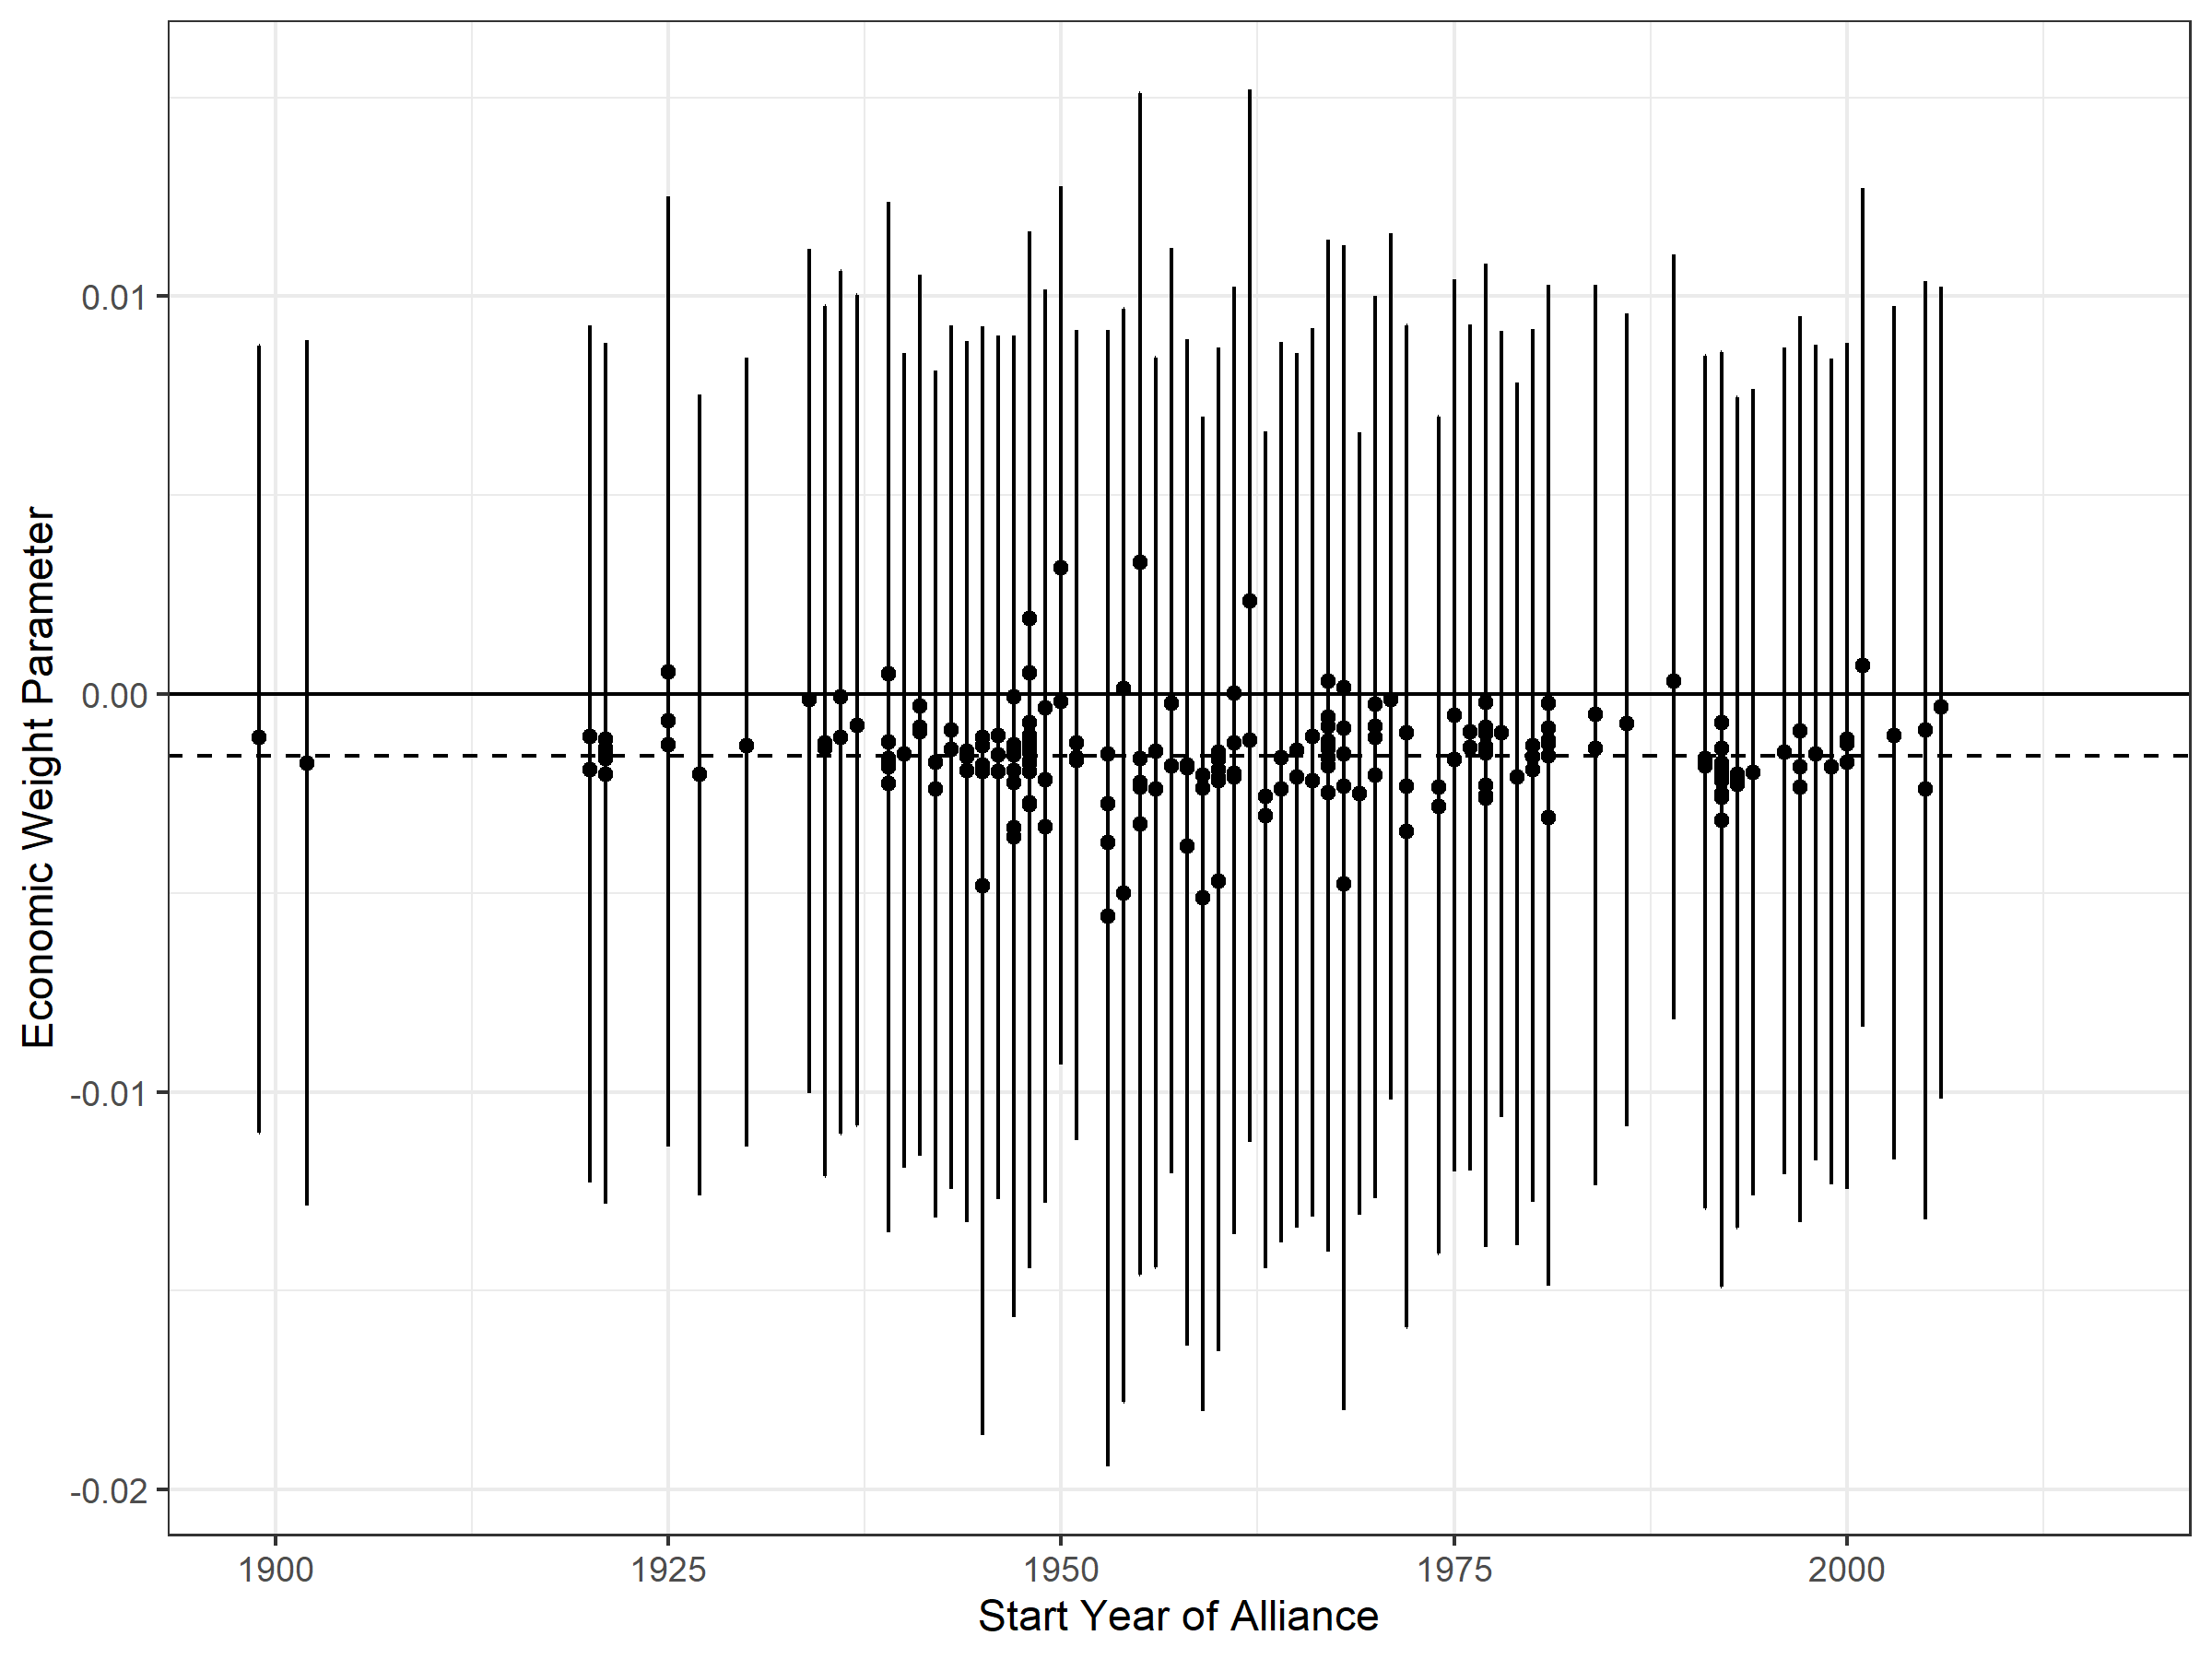
\includegraphics[width=0.95\textwidth]{alliance-coefs-year.png}
	\caption{Estimated association between economic weight and defense spending growth in 204 defensive and offensive alliances from 1919 to 2007. Positive estimates match the predictions of the public goods model. Points represent the posterior mean and the error bars cover the 90\% credible interval. The dashed line marks the posterior mean of the $\theta$ parameter, which is the average association between economic weight and percentage changes in military spending.}
	\label{fig:alliance-coefs-year}
\end{figure}


No alliances have a positive 90\% credible interval to match the public goods model's predictions. 
Most credible intervals are consistent with military spending growth between -0.02 to 0.015. 
Only 13 of the 204 alliances have a positive posterior mean. 
Therefore, there is little evidence of free-riding based on economic weight as the public goods model predicts. 

\textbf{
To give further evidence, I use the $\gamma$ parameters to predict the effect of participation in specific alliances for large and small states.
\autoref{fig:pred-sum} summarizes estimates for several notable alliances. 
Once again, there is limited evidence of lower defense spending by small states and higher spending by large states. 
Even alliances with the expected pattern of military spending across large and small members have uncertain predictions of military spending growth.  
}


\begin{figure}[htbp]
	\centering
		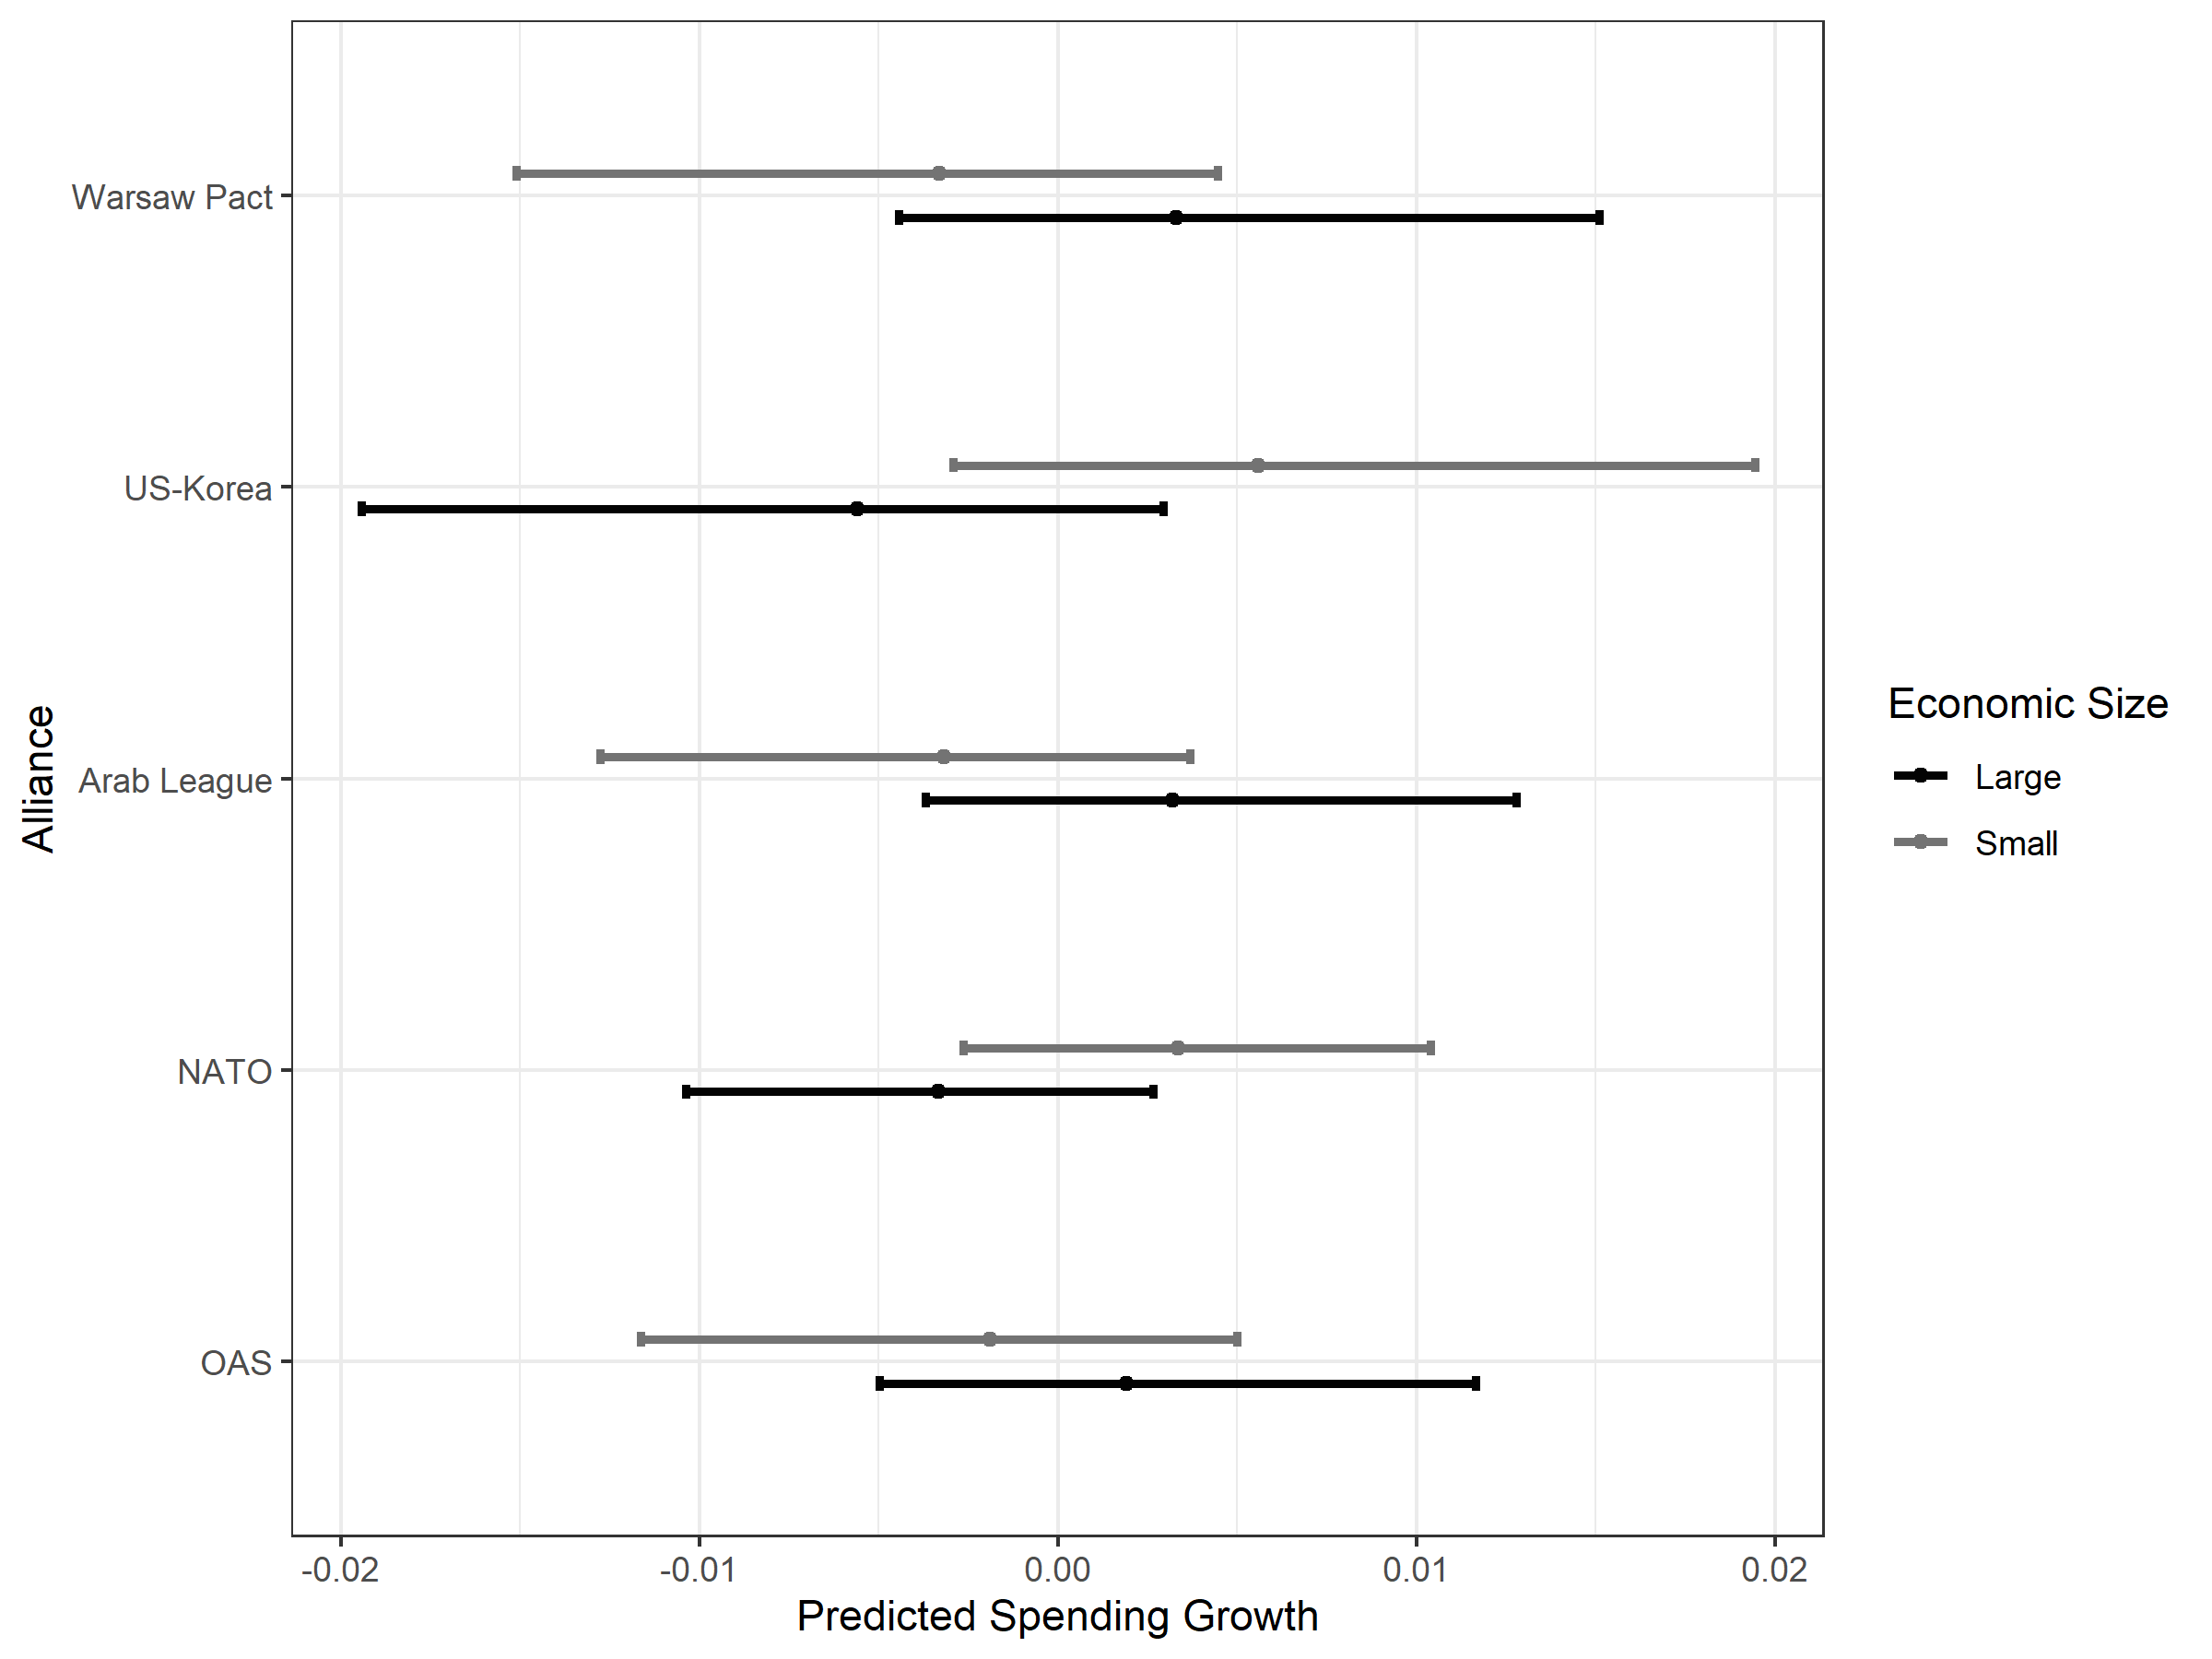
\includegraphics[width=0.95\textwidth]{pred-sum.png}
	\caption{Estimated impact of alliance participation on defense spending growth in large and small members of the OAS (ATOPID 3150), NATO (ATOPID 3180), the Arab League (ATOPID 3205), the U.S.-Korea alliance (ATOPID 3240) and the Warsaw Pact (ATOPID 3285). Points mark the mean estimated impact of alliance participation on military spending and the error bars cover the 90\% interval.}
	\label{fig:pred-sum}
\end{figure}

\textbf{
First, the NATO estimates in \autoref{fig:pred-sum} corroborate the size result of \citet{PluemperNeumayer2015}, as there is no evidence that small economic weight encourages lower military spending.
Expressing the impact of alliance participation through economic weight gives a small estimate of the impact of NATO participation on large and small members.  
Junior NATO members may still spend less on the military by relying on allied capability \citep{GeorgeSandler2017}, however. 
Furthermore, the U.S.-South Korea alliance (ATOPID 3240) estimates in \autoref{fig:pred-sum} are the reverse of the free-riding predictions. 
}

\textbf{
Among other alliances, the Arab League (ATOPID 3205), OAS (ATOPID 3150) and Warsaw Pact (ATOPID 3285) have the expected results for the public goods model, albeit with substantial uncertainty.
Although large alliance members increase spending and small members decrease spending in expectation, all these estimates are consistent with substantial positive and negative, as well as null effects. 
This suggests that highly asymmetric multilateral alliances are the most likely cases of free-riding, but that free-riding based on economic weight is weak even then.
There are no clear differences in military spending growth based on economic weight, even in some of the best-case alliances for the public goods model's free-riding predictions. 
}


\section{Conclusion}

% Add paragraph summarizing results
Although Olson and Zeckhauser's model is parsimonious, there is little evidence to match its prediction of free-riding based on economic weight. 
These results provide general evidence that economic weight is not a determinant of free-riding, which matches the finding of \citet{PluemperNeumayer2015} in NATO. 
The results do not rule out that alliances provide public goods, or that alliance participation reduces small states' military spending, however. 


If alliances do provide public goods, they may only do so in particular circumstances. 
Small states may only reduce military spending if they believe allied commitments are credible \citep{Goldstein1995, DigiuseppePoast2016}, or leaders are inclined to lower spending \citep{Fuhrmann2020}. 
If that is the case, inquiry should emphasize sources of leverage in bargaining between alliance members \citep{Morrow1991, Norrlof2010, Brooksetal2013, Johnson2015, Kim2016}. 
Alternatively, the extent to which security from an alliance is a public good may vary with factors like technology and strategic doctrine \citep{SandlerHartley2001}. 


Beyond scholarship, the results have implications for policymakers and pundits' inclination to use ``free-riding'' rhetoric in alliance politics. 
Free-riding is inextricable from a public goods understanding of alliances.
But without a clear sense of when or whether alliance provide public goods, free-riding is an inaccurate description of reduced defense effort by alliance participants.  
Low defense effort could reflect cheap-riding on allied capability, or efficiency gains from specialization in pooled military resources. 


Despite these results, collective action remains a central concept in international politics.   
It may be inappropriate to use alliances to understand collective action problems in international organizations more generally, as \citet[pg. 266-7]{OlsonZeckhauser1966} advocate, but collective action applies to other international organizations. 
Still, with little evidence of free-riding based on economic weight, policymakers and scholars should be cautious about relying on the public goods model to understand alliance politics.  



\singlespace


\bibliography{../../../MasterBibliography} 





\end{document}

